\chapter{Figure example formats}

FIGURE
\begin{figure}[H]
	\centering
	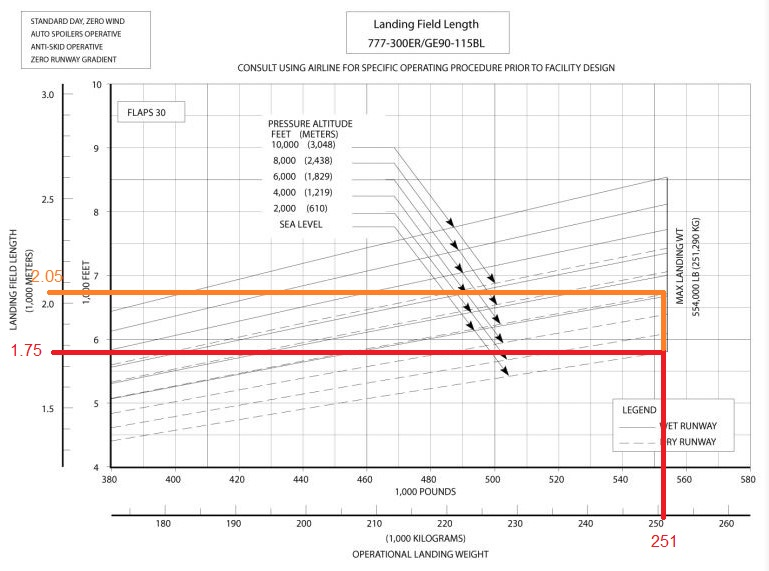
\includegraphics[clip, trim=0cm 0cm 0cm 0cm, width=0.95\textwidth]{./images/B777/landingdistance777}
	\caption{Landing distance vs MTOW for the Boeing 777.} %nom de la figura
	\label{} %per denotar una referencia
\end{figure}


TABLE
\begin{table}[htb]
	\centering
	\begin{tabular}{ll p{5cm}}
		\midrule[2pt]
		\(T_1\)& 13 cm\\
		\(T_2\) & 21 cm\\
		\(T_3\)& 62 cm \\
		\(T_t\)& 95 cm\\
		\bottomrule[2pt]
	\end{tabular}
	\caption{Thickness after the materials correction factor.}
	\label{}
\end{table}